\documentclass[../p116main.tex]{subfiles}
\graphicspath{{\subfix{../figures/}}}

\begin{document}

\chapter{Quantum States}
\section{Stern-Gerlach Experiments}
We'll begin our discussion of quantum mechanics with a classic experiment that has been used to measure the intrinsic spin angular momentum of an atom.
To get here, though, we first need to know how spin interacts with magnetic fields.
In classical mechanics, all angular momentum is orbital and has $\mbf{L} = \mbf{r} \times \mbf{p}$.
So for a charge-$q$, mass-$m$ point particle moving with speed $v$ in a circular orbit of radius $r$, the magnetic moment is
\[ \mu = \frac{I \cdot \pi r^2}{c} = \frac{1}{c} \frac{qv}{2\pi r} \cdot \pi r^2 = \frac{q}{2mc} L \;\implies\; \bm \mu = \frac{q}{2mc} \mbf{L}, \]
expressed in Gaussian units.
It turns out that the magnetic moment due to spin angular momentum $\mbf{S}$ is identical up to a unitless, experimentally-determined constant of proportionality $g$: $\bm \mu = (gq / 2mc) \mbf{S}$.

\parbox{0.85\textwidth}{
    There's another, much larger difference between orbital and spin angular momentum, though.
    Suppose we shoot a beam of silver atoms through the magnetic field generated by a pointed north pole and a flat south pole; a cross section of this arrangement (called a Stern-Gerlach device) is provided at right.
    We can see that this magnetic field is inhomogeneous.
    \vspace{6pt}

    Let the $+z$-direction point upward toward the south pole.
    When a neutral atom with magnetic moment $\bm \mu$ enters this device it experiences a force $\mbf{F} = \nabla (\bm \mu \cdot \mbf{B})$, the $z$-component of which is approximately $F_z \simeq \mu_z \cdot \partial B_z / \partial z$.
    Since the magnetic field gradient $\partial B_z / \partial z$ is negative, atoms with $\mu_z < 0$ are deflected upward and ones with $\mu_z > 0$ are deflected downward.
    \vspace{6pt}

    Now, if we were to capture all these deflected atoms on a plate on the other side of the SG$\mbf{z}$
}\parbox{0.15\textwidth}{
    \quad\;
    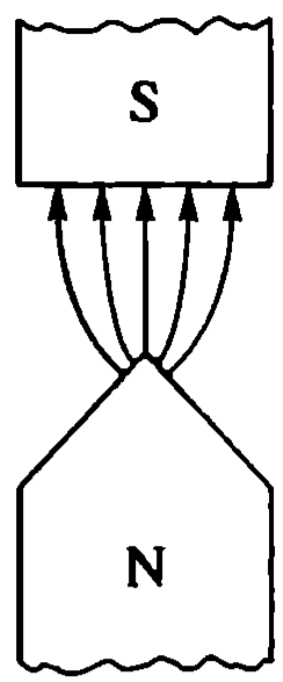
\includegraphics[width=0.1\textwidth]{sternGerlach.png}
}

\vspace{-4pt}
device, we might expect to see a continuum of deflections as $\bm \mu$ can be oriented all sorts of ways in space.
But this is not so---instead, the beam simply gets split into two.
This means that there are only two possibilities for $\mu_z$, and thus that there are only two possibilities for $S_z$.
Since the magnetic moment of a silver atom is largely due to a single electron, an electron must have exactly two spin states: $\hbar / 2$ (``spin up'') and $-\hbar / 2$ (``spin down'').
These deflect upward and downward, respectively.

We can leverage the fact that Stern-Gerlach devices split beams of particles according to their intrinsic spins to devise a few experiments, each of which reveals something important about quantum mechanics.
We'll use the ``ket vector'' shorthand $\ket{\pm \mbf{z}}$ to denote a particle with $S_z = \pm \hbar / 2$.
\begin{itemize}[topsep=0pt]
    \item A beam of particles in $\ket{+\mbf{z}}$ enters a SG$\mbf{z}$ device.
    We find that all particles exit still in $\ket{+\mbf{z}}$.

    \item A $\ket{+\mbf{z}}$ beam enters a SG$\mbf{x}$ device.
    Half of the particles exit in $\ket{+\mbf{x}}$, while the other half exit in $\ket{-\mbf{x}}$.

    \item A $\ket{+\mbf{z}}$ beam passes through a SG$\mbf{x}$ device, and the ones that end up in $\ket{+\mbf{x}}$ enter a SG$\mbf{z}$ device.
    Half of the particles exit in $\ket{+\mbf{z}}$, while the other half exit in $\ket{-\mbf{z}}$.
\end{itemize}
For the fourth experiment we employ a modified Stern-Gerlach device, which involves a set of four ``simple'' devices, two of which are upside-down.
The upside-down devices are squished between the other two so that particles passing through are split according to their spins and then brought back together again.
\begin{itemize}[topsep=0pt]
    \item A $\ket{+\mbf{z}}$ beam passes through a modSG$\mbf{x}$ device and then enter a SG$\mbf{z}$ device.
    All particles exit in $\ket{+\mbf{z}}$.
\end{itemize}
These experiments reveal that spin measurements change the state of the system.
In the third experiment none of the particles start with $\ket{-\mbf{z}}$, but by the end half of them are in this state.
We don't see this in the fourth experiment, though, since we never actually make any measurements!

This distinction suggests that probabilities don't tell the whole story here.
When we go to develop a formalism for quantum mechanics, we'll need to include some kind of ``interference'' that cancels out the $\ket{-\mbf{z}}$ state as the particles traverse the modSG\textbf{x} device.
In analogy with the relationship between an electromagnetic wave's intensity and its corresponding field amplitude, we'll soon introduce a ``probability amplitude'' that we can square to get a probability.
It will be these amplitudes, not the probabilities themselves, that we do calculations with when we make predictions in the quantum world.

\section{The Quantum State Vector}
We'll continue to constrain our attention primarily to spin for a while, as we begin building the mathematical foundations of quantum mechanics.
We will include more degrees of freedom in our quantum states later on, things like position and momentum; the principles here will generalize quite easily.

In our formalism the ket vector $\ket{+\mbf{z}}$ is more than just a shorthand for a spin-up state.
It is actually an element of an abstract vector space with basis $\left\{ \ket{+\mbf{z}}, \ket{-\mbf{z}} \right\}$.
So if we're given an arbitrary spin state $\ket{\psi}$, which we could generate by pointing a Stern-Gerlach device in an arbitrary direction, we could express the state as a linear combination of the basis states:
\[ \ket{\psi} = c_+ \ket{+\mbf{z}} + c_- \ket{-\mbf{z}}. \]
The fact that any state can be expressed as a superposition of $\ket{+\mbf{z}}$ and $\ket{-\mbf{z}}$ means that these two states comprise a complete set.
Now, a state $\ket{\psi}$ can also be represented with a bra vector
\[ \bra{\psi} = c_+' \bra{+\mbf{z}} + c_-' \bra{-\mbf{z}}. \]
The purpose of a bra $\bra{\varphi}$ is to meet with a ket $\ket{\psi}$ to form a bracket $\braket{\varphi}{\psi}$, which is a (complex) inner product that represents the amplitude that a particle in $\ket{\psi}$ will be measured in $\ket{\varphi}$.
We've seen from experiment that $\braket{-\mbf{z}}{+\mbf{z}} = 0$ and that $\braket{+\mbf{z}}{+\mbf{z}}$ is nonzero; we'll soon see that it is also crucial that all states satisfy $\braket{\psi}{\psi} = 1$ for a probabilistic interpretation of quantum mechanics to make sense.

By the distributivity of the inner product, we can deduce that
\begin{align*}
    \braket{+\mbf{z}}{\psi} &= c_+ \braket{+\mbf{z}}{+\mbf{z}} + c_- \braket{+\mbf{z}}{-\mbf{z}} = c_+, \qquad \braket{\psi}{+\mbf{z}} = c_+', \\
    \braket{-\mbf{z}}{\psi} &= c_+ \braket{-\mbf{z}}{+\mbf{z}} + c_- \braket{-\mbf{z}}{-\mbf{z}} = c_-, \qquad \braket{\psi}{-\mbf{z}} = c_-'.
\end{align*}
Also by distributivity, $\braket{\psi}{\psi} = \braket{\psi}{+\mbf{z}} \braket{+\mbf{z}}{\psi} + \braket{\psi}{-\mbf{z}} \braket{-\mbf{z}}{\psi} = 1$, so we must have $\braket{\psi}{\pm\mbf{z}} = \braket{\pm\mbf{z}}{\psi}^*$ to guarantee real terms.
It follows that $c_\pm' = c_\pm^*$.
Using this to rewrite the above gives
\[ \braket{\psi}{\psi} = c_+^* c_+ + c_-^* c_- = 1; \]
we therefore interpret $c_\pm^* c_\pm = \left| \braket{\pm \mbf{z}}{\psi} \right|^2$ as the probability of measuring $\ket{\pm \mbf{z}}$ from $\ket{\psi}$.
Thus in general a state isn't necessarily spin-up or spin-down at all, but rather is a superposition of these two states until a measurement of $S_z$ is taken.
The expectation value and uncertainty of such a measurement are given by
\[ \langle S_z \rangle = c_+^* c_+ (\hbar / 2) + c_-^* c_- (-\hbar / 2), \qquad (\Delta S_z)^2 = \langle (S_z - \langle S_z \rangle)^2 \rangle = \langle S_z^2 \rangle - \langle S_z \rangle^2. \]
Finally, we'll give a quick justification for why we must allow our probability amplitudes ot be complex.
Our experiments suggest that we have the kets
\[ \ket{+\mbf{x}} = \frac{e^{i \delta_+}}{\sqrt{2}} \ket{+\mbf{z}} + \frac{e^{i \delta_-}}{\sqrt{2}} \ket{-\mbf{z}}, \qquad \ket{+\mbf{y}} = \frac{e^{i \gamma_+}}{\sqrt{2}} \ket{+\mbf{z}} + \frac{e^{i \gamma_+}}{\sqrt{2}} \ket{+\mbf{z}}; \]
if we define $\delta = \delta_- - \delta_+$ and $\gamma = \gamma_- - \gamma_+$, some algebra reveals that
\[ \left| \braket{+\mbf{y}}{+\mbf{x}} \right|^2 = \frac{1}{2} \big( 1 + \cos(\delta - \gamma) \big). \]
To agree with the observation that $\left| \braket{+\mbf{y}}{+\mbf{z}} \right|^2$ we must have $\delta - \gamma = \pm \pi / 2$, and no matter which we take we will get complex basis coefficients!
The standard is $\delta = 0$, $\gamma = \pi / 2$, and $\delta_+ = \gamma_+ = 0$ so that
\[ \ket{+\mbf{x}} = \frac{1}{\sqrt{2}} \ket{+\mbf{z}} + \frac{1}{\sqrt{2}} \ket{-\mbf{z}}, \quad \ket{+\mbf{y}} = \frac{1}{\sqrt{2}} \ket{+\mbf{z}} + \frac{i}{\sqrt{2}} \ket{-\mbf{z}}. \]
The spin-down kets are simply the normalized orthogonal states
\[ \ket{-\mbf{x}} = \frac{1}{\sqrt{2}} \ket{+\mbf{z}} - \frac{1}{\sqrt{2}} \ket{-\mbf{z}}, \quad \ket{-\mbf{y}} = \frac{1}{\sqrt{2}} \ket{+\mbf{z}} - \frac{i}{\sqrt{2}} \ket{-\mbf{z}}, \]
and we could use our knowledge of $\braket{\pm \mbf{x}}{\pm \mbf{z}}$ and $\braket{\pm \mbf{y}}{\pm \mbf{z}}$ to write $\ket{\pm \mbf{z}}$ in terms of these kets.

\section{Rotation and Projection Operators}
We'll very often find ourselves in positions where we need to transform one quantum state into another.
One way we might do this is by applying a rotation operator $\hat R(\phi \mbf{k})$ to a ket, which rotates its corresponding three-vector through an angle $\phi$ about the $z$-axis.
For example, $\hat R(\frac{\pi}{2} \mbf{k}) \ket{+\mbf{x}} = \ket{+\mbf{y}}$.
In order to act on a bra we must define a new operator $\hat R^\dagger$, called its adjoint; this allows us to satisfy, say,
\[ 1 = \braket{+\mbf{x}}{+\mbf{x}} = \bra{+\mbf{z}} \hat R^\dagger \left( \frac{\pi}{2} \mbf{j} \right) \hat R \left( \frac{\pi}{2}\mbf{j} \right) \ket{+\mbf{z}} = \braket{+\mbf{z}}{+\mbf{z}}, \]
so long as $\hat R^\dagger \hat R = 1$.
Such an operator is called a unitary operator, and so $\hat R$ must be unitary in order to conserve probability.
Now, in giving a more explicit definition for $\hat R$, we'll find it useful to define an infinitesimal
\[ \hat R(d\phi \, \mbf{k}) = 1 - \frac{i}{\hbar} \hat J_z d\phi, \]
where $\hat J_z$ is an operator that ``generates'' rotations about the $z$-axis.
Roughly speaking, it tells the quantum state vector how, exactly, to move through space to reflect a small nudge in three-space.
The finite rotation operator is then given by
\[ \hat R(\phi \mbf{k}) = \lim_{N \to \infty} \left[ 1 - \frac{i}{\hbar} \hat J_z \left( \frac{\phi}{N} \right) \right]^{N} = e^{-i \hat J_z \phi / \hbar}. \]
The rotation generator $\hat J_z$ has a few nice properties that will help us physically identify it.
For one,
\[ 1 = \hat R^\dagger (d\phi \, \mbf{k}) \hat R (d\phi \, \mbf{k}) = \left( 1 + \frac{i}{\hbar} \hat J_z^\dagger d\phi \right) \left( 1 - \frac{i}{\hbar} \hat J_z d\phi \right) = 1 + \frac{i}{\hbar} (\hat J_z^\dagger - \hat J_z) d\phi + O(d\phi^2), \]
meaning $\hat K_z^\dagger = \hat J_z$; we therefore call $\hat J_z$ Hermitian (or self-adjoint).
We can also deduce its eigen-things---by Taylor-expanding $\hat R$,
\[ \hat R(\phi \mbf{k}) = 1 - \frac{i\phi \hat J_z}{\hbar} + \frac{1}{2!} \left( -\frac{i\phi \hat J_z}{\hbar} \right)^2 + \cdots, \]
we can immediately see that its eigenkets are $\ket{\pm \mbf{z}}$ since no other ket would yield an eigenvalue equation.
We can also see that having respective eigenvalues of $\pm \hbar / 2$ would yield $\hat R(\phi \mbf{k}) \ket{\pm \mbf{z}} = e^{\mp i\phi / 2} \ket{\pm \mbf{z}}$, meaning $\hat R$ changes the states only by an overall phase (so effectively not at all).     % NOTE: a rotation through phi = 2pi causes a state to flip phase
Comparing this with the result of the Stern-Gerlach experiment allows us to identify $\hat J_z$ with the angular momentum in the $z$-direction!

We'll also find it useful to define a pair of projection operators, $\hat P_\pm = \ket{\pm \mbf{z}} \bra{\pm \mbf{z}}$, which project the components of a ket along $\ket{\pm \mbf{z}}$.
Its eigenkets are $\ket{\pm \mbf{z}}$ with eigenvalues 1 and 0, depending on which operator we're using, and the identities $\hat P_\pm^2 = \hat P_\pm$ and $\hat P_\pm \hat P_\mp = 0$ have nice geometric intuition.

More essential to our future discussion, however, is to define an identity (``do-nothing'') operator
\[ 1_z = \ket{+\mbf{z}} \bra{+\mbf{z}} + \ket{-\mbf{z}} \bra{-\mbf{z}}, \]
which reflects how the kets $\ket{+\mbf{z}}$ and $\ket{-\mbf{z}}$ form a complete basis of spin states.
(We specify $1_z$ to emphasize that we're writing the identity $1$ in the $S_z$-basis.)
We'll soon see how useful it is to insert the identity into different places to illuminate new things about the expressions we write!

Take our fourth Stern-Gerlach experiment, for example.
The modSG\textbf{x} device there acts as the identity operator as it does not modify the incoming $\ket{+\mbf{z}}$ state, so the amplitude of measuring $\ket{-\mbf{z}}$ vanishes---that is, $\braket{-\mbf{z}}{+\mbf{z}} = 0$.
But to illuminate more about the situation we can insert the identity $1_x$ into the bracket:
\begin{align*}
    \braket{-\mbf{z}}{+\mbf{z}} &= \bra{-\mbf{z}} \Big( \ket{+\mbf{z}}\bra{+\mbf{z}} + \ket{-\mbf{z}}\bra{-\mbf{z}} \Big) \ket{+\mbf{z}} \\
    &= \braket{-\mbf{z}}{+\mbf{x}} \braket{+\mbf{x}}{+\mbf{z}} + \braket{-\mbf{z}}{-\mbf{x}} \braket{-\mbf{x}}{+\mbf{z}}.
\end{align*}
This hearkens back to the laws of probability we're familiar with.
Each term represents the amplitude that a particle takes a particular ``path'' through the modSG\textbf{x} device (and so we add them), while each factor represents a particular ``step'' in each of these paths (and so we multiply them).

\section{Matrix Mechanics}
We will find it convenient to represent kets $\ket{\psi} = c_+ \ket{+\mbf{z}} + c_- \ket{-\mbf{z}}$ using column vectors and their corresponding bras using row vectors:
\[ \ket{\psi} \xrightarrow[{S_z \,\textrm{basis}}]{} \begin{bmatrix} c_+ \\ c_- \end{bmatrix}, \qquad \bra{\psi} \xrightarrow[{S_z \textrm{ basis}}]{} \begin{bmatrix} c_+^* & c_-^* \end{bmatrix}. \]
In this way, brackets are represented by simple matrix multiplication.
Note that this representation of a quantum state is dependent on what basis we choose to write it in---if we were to choose the $S_x$-basis, for example, the components would be very different.

If kets are represented by column vectors, then operators are represented by matrices that act on those column vectors (and their adjoints are their conjugate transposes).
These representations, of course, are also basis-dependent; for example,
\[ \hat A \ket{\psi} \xrightarrow[{S_z \,\textrm{basis}}]{}\begin{bmatrix} \bra{+\mbf{z}} \hat A \ket{\psi} \\ \bra{-\mbf{z}} \hat A \ket{\psi} \end{bmatrix} = \begin{bmatrix} \bra{+\mbf{z}} \hat A \ket{+\mbf{z}} & \bra{+\mbf{z}} \hat A \ket{-\mbf{z}} \\ \bra{-\mbf{z}} \hat A \ket{+\mbf{z}} & \bra{-\mbf{z}} \hat A \ket{-\mbf{z}} \end{bmatrix} \begin{bmatrix} \braket{+\mbf{z}}{\psi} \\ \braket{-\mbf{z}}{\psi} \end{bmatrix}. \]
There's a couple of ways we could've arrived here.
Mathematically, we've inserted the identity operator $1_x$ between $\hat A$ and $\ket{\psi}$ in each component.
Geometrically, we can see that each column of the matrix is simply the column-vector representation of $\hat A \ket{\pm \mbf{z}}$ in the $S_z$-basis.

This representation suggests that we can view our operators from a couple of different perspectives.
On one hand we might view $\hat A$ as operating to the left and literally modifying the quantum state; this is called an active transformation.
But on the other, $\hat A$ may operate to the left and perform the adjoint (inverse) transformation to the basis states; this is called a passive transformation.
For example, for two kets related by $\ket{\psi'} = \hat R^\dagger (\frac{\pi}{2} \mbf{j}) \ket{\psi}$ we can write
\[ \ket{\psi'} \xrightarrow[{S_z \,\textrm{basis}}]{} \begin{bmatrix} \braket{+\mbf{z}}{\psi'} \\ \braket{-\mbf{z}}{\psi'} \end{bmatrix} = \begin{bmatrix} \bra{+\mbf{z}} \hat R^\dagger (\frac{\pi}{2} \mbf{j}) \ket{\psi} \\ \bra{-\mbf{z}} \hat R^\dagger (\frac{\pi}{2} \mbf{j}) \ket{\psi} \end{bmatrix} = \begin{bmatrix} \braket{+\mbf{x}}{\psi} \\ \braket{-\mbf{x}}{\psi} \end{bmatrix} \xleftarrow[{S_z \,\textrm{basis}}]{} \ket{\psi}, \]
where we've temporarily defined $\ket{+\mbf{x}} = \hat R (\frac{\pi}{2} \mbf{j}) \ket{+\mbf{z}}$ and $\ket{-\mbf{x}} = \hat R (\frac{\pi}{2} \mbf{j}) \ket{-\mbf{z}}$ for convenience.
We can use these passive transformations to perform changes of basis on kets,
\begin{align*}
    \begin{bmatrix} \braket{+\mbf{x}}{\psi} \\ \braket{-\mbf{x}}{\psi} \end{bmatrix} &= \begin{bmatrix} \bra{+\mbf{z}} \hat R^\dagger (\frac{\pi}{2} \mbf{j}) \ket{+\mbf{z}} & \bra{+\mbf{z}} \hat R^\dagger (\frac{\pi}{2} \mbf{j}) \ket{-\mbf{z}} \\ \bra{-\mbf{z}} \hat R^\dagger (\frac{\pi}{2} \mbf{j}) \ket{+\mbf{z}} & \bra{-\mbf{z}} \hat R^\dagger (\frac{\pi}{2} \mbf{j}) \ket{-\mbf{z}} \end{bmatrix} \begin{bmatrix} \braket{+\mbf{z}}{\psi} \\ \braket{-\mbf{z}}{\psi} \end{bmatrix}, \\
    \intertext{but for computations it may be more convenient to simply insert $1_x$ between $\bra{\pm \mbf{x}}$ and $\ket{\psi}$:}
    &= \begin{bmatrix} \braket{+\mbf{x}}{+\mbf{z}} & \braket{+\mbf{x}}{-\mbf{z}} \\ \braket{-\mbf{x}}{+\mbf{z}} & \braket{-\mbf{x}}{-\mbf{z}} \end{bmatrix} \begin{bmatrix} \braket{+\mbf{z}}{\psi} \\ \braket{-\mbf{z}}{\psi} \end{bmatrix}.
\end{align*}
We will denote this matrix by $\mathbb S_{x \leftarrow z} = \mathbb S_{z \leftarrow x}^\dagger$.
Note that $\mathbb S$ is unitary for all bases, since it is simply the matrix representation of a rotation operator.
We can also do change of basis on operators:
\[ \hat A \xrightarrow[{S_x \,\textrm{basis}}]{} \mathbb S_{z \leftarrow x}^\dagger \mathbb A_z \mathbb S_{z \leftarrow x}, \]
where $\mathbb A_z$ is the representation of $\hat A$ in the $S_z$-basis.
Mathematically, we have inserted $1_x 1_z$ and $1_z 1_x$ before and after $\mathbb A_{z}$; geometrically, we are ``rotating'' into the $S_z$-basis, performing $\hat A$, and then rotating back.

We can use matrix mechanics to determine expectation values, too.
For example, we can write
\[ \langle S_z \rangle = \bra{\psi} \hat J_z \ket{\psi}. \]
It's clear why this works when we're working in the $\hat J_z$-eigenbasis, since in this case the matrix representation is diagonal with eigenvalue entries.
But the great thing about expressing expectation values in this way is that it doesn't matter what representation we use---as long as we're consistent, we'll get the correct value!

Now, what we've done here applies to any two-state system.
For example, we can also represent the polarization of a photon using two orthogonal basis states $\ket{\bi x}$ and $\ket{\bi y}$.
Experiment suggests that rotating through a counterclockwise angle $\phi$ gives \vspace{-10pt}
\begin{align*}
    \ket{\bi x'} &= \phantom{-}\cos \phi \, \ket{\bi x} + \sin \phi \, \ket{\bi y}, \\
    \ket{\bi y'} &= -\sin \phi \, \ket{\bi x} + \cos \phi \, \ket{\bi y}.
\end{align*}
Note that we could have derived this from the geometry of projecting the primed states onto the unprimed ones.
From here we could get the matrix that transforms from the unprimed basis to the primed one!

\pagebreak

Lastly, in order to encode circular polarization we define
\[ \ket{\bi R} = \frac{1}{\sqrt{2}} \big( \ket{\bi x} + i \ket{\bi y} \big), \qquad \ket{\bi L} = \frac{1}{\sqrt{2}} \big( \ket{\bi x} - i \ket{\bi y} \big). \]
If we were to rotate these through a counterclockwise angle $\phi$ about the $z$-axis, we'd find that $\ket{\bi R'} = e^{-\phi} \ket{\bi R}$ and $\ket{\bi L'} = e^{i\phi} \ket{\bi L}$.
This means that these must be eigenstates of $\hat J_z$,this time with eigenvalues $\pm \hbar$!
This reflects how photons are spin-1 particles (and, because they're massless, how they cannot have spin 0).

At this point we've hinted at all the key postulates of quantum mechanics.
\begin{itemize}[topsep=0pt]
    \item We will describe the state of a quantum system as a vector in some abstract ``Hilbert space'';
    \item each observable $A$ of such a system will correspond to a Hermitian operator $\hat A$;
    \item the eigenstates of this operator are those states with definite $A$ and the corresponding eigenvalues are the results of measuring $A$; and
    \item the symmetries of such a system will correspond to unitary operators generated by their respective Noether quantity.
\end{itemize}
Formalism in hand, it's time to dive into the physics!

\end{document}